\section{The LEDGER Audit Layer}\label{sec:method}

\begin{figure*}[t]
\centering
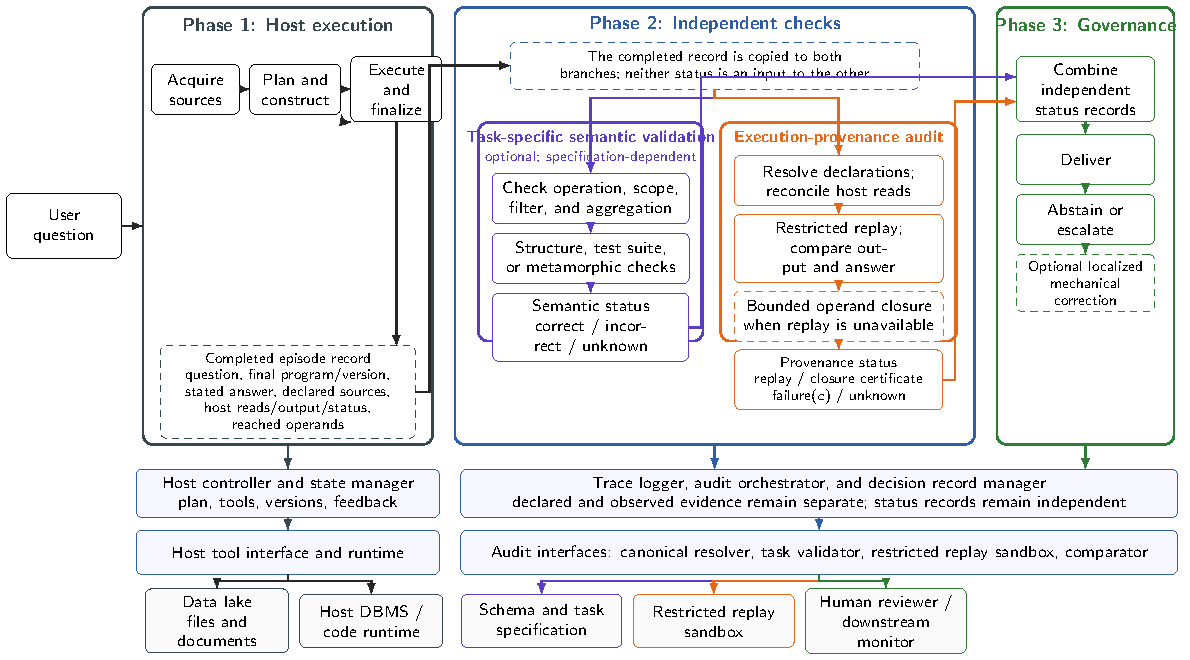
\includegraphics[width=0.99\textwidth]{fig_architecture.pdf}
\caption{LEDGER consumes a completed episode after host execution. Semantic validation and execution-provenance auditing run independently; dashed boxes denote the bounded fallback and an optional correction path that is not evaluated here.}
\label{fig:architecture}
\end{figure*}

\subsection{Overview and trace capture}

The host wrapper records program revisions, the final program snapshot, stdout, exceptions, declared citations, runtime data reads, accessed columns, and scalar operands reaching the final expression. Paths and dataset identifiers are canonicalized before comparison. Declared sources, host reads, and replay reads remain separate fields throughout the audit record.

For dataframe programs, operand attribution follows accessed columns and scalar values that reach the final expression. For SQL, the record stores relations, projected attributes, predicates, aggregates, and returned scalars. Each outcome carries a concise evidence string and the machine-readable artifact needed to reproduce it.

\subsection{Episode audit and failure precedence}\label{sec:auditproc}

Algorithm~\ref{alg:audit} implements the complete audit. Evidence-boundary failures take precedence over replay failures, which take precedence over output mismatch. When several violations are observed, the record preserves the full set and exposes the earliest class as the primary outcome. Closure is consulted only when no explicit failure has been observed and the final runtime is unavailable.

\begin{algorithm}[t]
\caption{LEDGER episode audit}
\label{alg:audit}
\begin{algorithmic}[1]
\Require episode $E$, resolver $R$, sandbox $H$, comparator $\operatorname{cmp}$, operations $\opset$, depth $d$
\State $F_{\mathrm{res}}\gets R(F_{\mathrm{decl}})$
\If{some declaration is unresolved}
  \State \Return $\failure(\mathrm{unresolved\ source})$
\EndIf
\If{$F_{\mathrm{host}}\nsubseteq F_{\mathrm{res}}$}
  \State \Return $\failure(\mathrm{undeclared\ host\ read})$
\EndIf
\If{$s_{\mathrm{host}}\neq\mathrm{success}$ and an answer was stated}
  \State \Return $\failure(\mathrm{host\ execution})$
\EndIf
\If{$P^*$ is runnable in $H$}
  \State $(F_{\mathrm{replay}},s_{\mathrm{replay}},v_{\mathrm{replay}})\gets\operatorname{Replay}(P^*,H[F_{\mathrm{res}}])$
  \If{$F_{\mathrm{replay}}\nsubseteq F_{\mathrm{res}}$}
    \State \Return $\failure(\mathrm{replay\ boundary})$
  \ElsIf{$s_{\mathrm{replay}}\neq\mathrm{success}$}
    \State \Return $\failure(\mathrm{replay\ execution})$
  \ElsIf{$v_{\mathrm{replay}}$ is not comparable}
    \State \Return $\failure(\mathrm{missing\ output})$
  \ElsIf{$\operatorname{cmp}(v_{\mathrm{replay}},\hat a;\tol)=1$}
    \State \Return $\cert_{\mathrm{replay}}$ and replay witness
  \Else
    \State \Return $\failure(\mathrm{output\ mismatch})$
  \EndIf
\EndIf
\If{reached operands are complete}
  \State \Return \Call{BoundedClosure}{$\operands,\opset,d,\hat a$}
\EndIf
\State \Return $\unknown$
\end{algorithmic}
\end{algorithm}

\subsection{Citation-restricted replay}

The replay sandbox mounts only $F_{\mathrm{res}}$, fixes deterministic library settings when available, and records every data read. The comparator normalizes strings, booleans, ordered or unordered lists, and numeric values under relative tolerance $\tol$. A successful certificate therefore binds a concrete program snapshot, a canonical evidence view, and a comparable output. Failure records retain the denied read, exception, missing output, or mismatching value that caused the decision.

\subsection{Operand-constrained fallback}\label{sec:closure}

Some archived episodes expose operands and a stated value while the original runtime is unavailable. Let
\[
\opset=\{\mathrm{sum,diff,ratio,pctchg,prod}\}.
\]
Starting from the trace-local operand multiset $\operands$, the depth-$d$ closure $\cl_d(\operands)$ recursively applies valid operations in $\opset$ with normalization and duplicate removal.

\begin{definition}[Closure certificate]\label{def:closure}
Episode $E$ receives a depth-$d$ closure certificate when $\hat a\in\cl_d(\operands)$ within tolerance $\tol$. The witness stores a minimal expression and its operand subset.
\end{definition}

\begin{algorithm}[t]
\caption{Bounded operand closure}
\label{alg:closure}
\begin{algorithmic}[1]
\Function{BoundedClosure}{$\operands,\opset,d,\hat a$}
\State $S_0\gets\operatorname{normalize}(\operands)$
\For{$j=1,\ldots,d$}
  \State $S_j\gets S_{j-1}$
  \ForAll{$x,y\in S_{j-1}$ and $o\in\opset$}
    \State add valid normalized $o(x,y)$ with an expression witness
  \EndFor
\EndFor
\If{$\hat a\in S_d$ within $\tol$}
  \State \Return $\cert_{\mathrm{closure}}$ and a minimal witness
\EndIf
\State \Return $\unknown$
\EndFunction
\end{algorithmic}
\end{algorithm}

\begin{proposition}[Closure completeness]\label{prop:complete}
If $\hat a$ is generated from reached operands by operations in $\opset$, expression depth at most $d$, and the audit's normalization and tolerance, then $\hat a\in\cl_d(\operands)$.
\end{proposition}
\noindent\emph{Proof sketch.} Leaves occur in $S_0$. Induction on expression depth places each valid internal result in the next closure level. The root therefore appears by depth $d$; The full proof appears in~\ref{app:proofs}.

The operating point is calibrated on 60 disjoint ConvFinQA examples and frozen at $d=2$ with relative tolerance $10^{-4}$. Context-wide numbers, held-out examples, and human labels do not change this setting.

\subsection{Semantic interface and governance decision}\label{sec:semanticinterface}

The audit record exposes $q$, $P^*$, schema references, and replay output to the optional validator $V_q$. SQL tasks permit normalized-structure comparison and execution on generated database variants \citep{zhong2020testsuite}; other deployments may supply executable constraints, metamorphic relations, a model-based judge, or human review. The resulting semantic status is appended to the audit record without modifying its provenance outcome.

A conservative decision policy delivers a provenance-certified answer when the semantic status is correct or unavailable under the deployment policy, and escalates semantically rejected or provenance-incomplete episodes. A uniquely localized mechanical mismatch can support an optional correction workflow; the present evaluation measures delivery and escalation and does not evaluate automated repair.



\begin{remark}
The provenance witness remains valid without a semantic validator. Semantic status is a separate, deployment-specific property.
\end{remark}

\subsection{Complexity and deterministic contract}

Resolution and read reconciliation cost $O(|F_{\mathrm{decl}}|+|F_{\mathrm{host}}|)$. Replay adds one execution of the final program. If $N_j$ is the number of closure candidates before duplicate removal, $m=|\operands|$, and $r=|\opset|$, then $N_d\le m+r\sum_{j=1}^{d}N_{j-1}^2$. Restricting $S_0$ to reached operands reduces every recursive expansion. For a fixed trace, resolver, runtime, comparator, normalization, and depth, the provenance audit is deterministic and invokes no language model.

\begin{table}[!t]
\centering
\caption{Interface between independent statuses and downstream action.}
\label{tab:policy}
\scriptsize
\begin{tabular}{@{}lll@{}}
\toprule
Provenance status & Semantic status & Default action \\
\midrule
certificate & correct & deliver \\
certificate & unknown & deliver or review by policy \\
certificate & incorrect & abstain / escalate \\
failure or unknown & any & abstain / escalate \\
localized mismatch & correct/unknown & optional correction \\
\bottomrule
\end{tabular}
\end{table}
